\newcommand{\model}{%
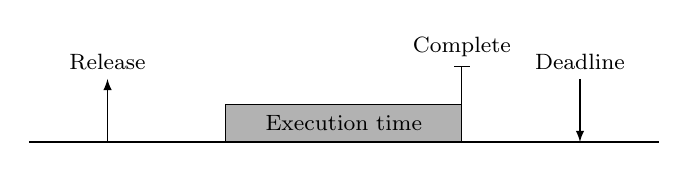
\begin{tikzpicture}[
  yscale = 0.8,
  normal/.style={fill=black!30},
  release/.style={-latex},
  complet/.style={-|},
  every text node part/.style={align=center}
]
%general params
\def\th{.6} %task height
\def\blockdim{(.4,.4)}
\def\arrowdim{(0,.5)}
\def\arrowdimB{(0,.4)}

%axes
\draw[thick, black] (0,0) -- (8, 0);

%L1
\draw[release] (1, 0) -- +(0,1) node[above] {{\footnotesize Release}};
\draw[normal]  (2.5, 0) rectangle +(3, \th) node[midway] {{\footnotesize Execution time}};
\draw[complet] (5.5, 0) -- +(0, 1.2) node[above] {{\footnotesize Complete}};
\draw[release] (7, 1) node[above] {{\footnotesize Deadline}} -- (7,0);

\end{tikzpicture}
}
